% ===================================================================
%  《月之都——〈广寒宫残简〉辑佚与考释》专用版式
%
%  丛书基座在 ../../shared/style/series-base.tex；本书只在这里追加
%  本书特有的东西。跨书共用的东西一律改基座，不要改这里。
% ===================================================================

% ===================================================================
%  远东异端史料与文明起源重构丛书 · 版式基座（series-base）
%
%  兄弟书目共用此文件。改这里 = 改全套书。
%  各书在自己的 preamble.tex 里 \input 本文件，再追加本书特有的定义。
%
%  体例：仿苏式/中译社科类古籍。16 开 185×260 mm，版心 147×214 mm。
%  依赖：XeLaTeX + ctex + xeCJK + zhnumber + Noto Serif/Sans CJK SC
% ===================================================================

\usepackage{geometry}
\geometry{
  paperwidth=185mm, paperheight=260mm,
  inner=21mm, outer=17mm, top=22mm, bottom=24mm,
  headheight=24pt, headsep=6.5mm, footskip=11mm
}

\usepackage{fontspec}
\usepackage{xeCJK}
\usepackage{xcolor}
\usepackage{graphicx}
\usepackage{array,tabularx,booktabs,multirow,makecell}
\usepackage{longtable}
\usepackage{multicol}
\usepackage{calc}
\usepackage{amsmath,amssymb}
\usepackage{enumitem}
\usepackage{fancyhdr}
\usepackage{titlesec}
\usepackage{titletoc}
\usepackage{tcolorbox}
\tcbuselibrary{skins,breakable}
\usepackage[perpage]{footmisc}
\usepackage{etoolbox}
\usepackage{eso-pic}
\usepackage{tikz}
\usetikzlibrary{patterns,arrows.meta,calc,positioning,decorations.pathmorphing,
                decorations.markings,shapes.geometric}
\usepackage{pgfplots}
\pgfplotsset{compat=1.17}
\usepackage{caption}
\usepackage[hidelinks,bookmarksnumbered,bookmarksopen]{hyperref}

% ---------------------------------------------------------------- 颜色
\definecolor{ink}{HTML}{17191C}
\definecolor{graphite}{HTML}{3F454C}
\definecolor{pencil}{HTML}{5B6167}
\definecolor{rulegrey}{HTML}{8B8F93}
\definecolor{faintgrey}{HTML}{C9C9C4}
\definecolor{oxblood}{HTML}{6E1B22}
\definecolor{coverbg}{HTML}{1A1C20}
\definecolor{coverink}{HTML}{E6DFCF}
\definecolor{coverdim}{HTML}{7C7A73}
\definecolor{shade}{HTML}{F2F0EA}
\definecolor{stamp}{HTML}{8C2B2B}

\color{ink}

% ---------------------------------------------------------------- 字体
\setmainfont{NotoSerif}[
  Extension=.ttf,
  UprightFont=*-Regular,
  BoldFont=*-Bold,
  ItalicFont=*-Italic,
  BoldItalicFont=*-BoldItalic,
  Path=/usr/share/fonts/noto/
]
\setsansfont{NotoSans}[
  Extension=.ttf,
  UprightFont=*-Regular,
  BoldFont=*-Bold,
  ItalicFont=*-Italic,
  BoldItalicFont=*-BoldItalic,
  Path=/usr/share/fonts/noto/
]
\setmonofont{JetBrains Maple Mono}[
  UprightFont=* Regular, BoldFont=* Bold, Scale=0.92
]

\setCJKmainfont{Noto Serif CJK SC}[
  BoldFont=Noto Serif CJK SC Bold,
  ItalicFont=Noto Serif CJK SC,
  BoldItalicFont=Noto Serif CJK SC Bold
]
% 让罗马数字、带圈数字等“类汉字”符号使用中文字体
\xeCJKDeclareCharClass{CJK}{"2150 -> "218F, "2460 -> "24FF, "3000 -> "303F}

% 标点用开明式：行首禁则与压缩都较默认的 plain 更稳，可减少「句号独行」。
\AtBeginDocument{\xeCJKsetup{PunctStyle=kaiming}}

\setCJKsansfont{Noto Sans CJK SC}[BoldFont=Noto Sans CJK SC Bold]
\setCJKmonofont{Noto Sans Mono CJK SC}

% 伪斜体的字距（中文无真斜体，此处仅作强调标记）
\newcommand{\jia}{\CJKfontspec{Noto Serif CJK SC}}

% ---------------------------------------------------------------- 版心
\linespread{1.42}
\setlength{\parindent}{2em}
\setlength{\parskip}{0pt}
\raggedbottom
\setlength{\emergencystretch}{2em}
\clubpenalty=10000
\widowpenalty=10000

% ---------------------------------------------------------------- 计数
\renewcommand{\thechapter}{\chinese{chapter}}
\renewcommand{\thesection}{\chinese{section}}
\renewcommand{\thesubsection}{\chinese{subsection}}
\renewcommand{\thefigure}{\arabic{chapter}-\arabic{figure}}
\renewcommand{\thetable}{\arabic{chapter}-\arabic{table}}
\renewcommand{\theequation}{\arabic{chapter}-\arabic{equation}}

% ---------------------------------------------------------------- 章标题
\newcommand{\chapterornament}{%
  \vspace{0.8\baselineskip}%
  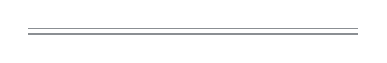
\begin{tikzpicture}[baseline=0pt]
    \fill[rulegrey] (0,0) rectangle (42mm,0.75pt);
    \fill[rulegrey] (0,2.4pt) rectangle (42mm,2.75pt);
  \end{tikzpicture}}

\titleformat{\chapter}[display]
  {\centering\normalfont}
  {\large\mdseries 第\,\thechapter\,章}
  {0.55\baselineskip}
  {\normalfont\LARGE\bfseries\linespread{1.15}\selectfont}
  [\chapterornament]
\titlespacing*{\chapter}{0pt}{-16pt}{30pt}

\titleformat{\section}
  {\normalfont\sffamily\large\bfseries\linespread{1.2}\selectfont}
  {第\,\thesection\,节}{0.6em}{}
\titlespacing*{\section}{0pt}{18pt}{9pt}

\titleformat{\subsection}
  {\normalfont\normalsize\bfseries}
  {\thesubsection、}{0.2em}{}
\titlespacing*{\subsection}{0pt}{13pt}{6pt}

\titleformat{\subsubsection}
  {\normalfont\normalsize\itshape}
  {}{0pt}{}
\titlespacing*{\subsubsection}{0pt}{10pt}{4pt}

% 章题下的俄文原题
\newcommand{\chaptersubtitle}[2]{%
  \begin{center}
  \vspace{-14pt}
  {\small\sffamily\color{pencil}#1}\\[2pt]
  {\small\sffamily\itshape\color{pencil}#2}
  \end{center}
  \vspace{4pt}
}

% 章前题记
\newcommand{\epigraphbox}[2]{%
  \begingroup
  \vspace{2pt}
  \begin{list}{}{\leftmargin=3.2em \rightmargin=2.2em \topsep=0pt
                 \parsep=0pt \itemsep=0pt}
  \item\relax
  {\small\linespread{1.32}\selectfont\color{ink!88}#1\par}
  \vspace{3pt}
  {\small\raggedleft\color{pencil}#2\par}
  \end{list}
  \vspace{6pt}
  \endgroup
}

% ---------------------------------------------------------------- 页眉页脚
% 注意：fancyhdr v5 的 \fancypagestyle 在使用时会执行其中的 \fancyhf{}，
% 从而清空全局 fancy 设置。故此处直接定义 \ps@ 样式，绕开该机制。
\makeatletter
\def\ps@frontmatterpage{%
  \let\@mkboth\@gobbletwo
  \let\@oddhead\@empty \let\@evenhead\@empty
  \def\@oddfoot{\hfil\small\thepage\hfil}%
  \def\@evenfoot{\hfil\small\thepage\hfil}}
\def\ps@plain{%
  \let\@mkboth\@gobbletwo
  \let\@oddhead\@empty \let\@evenhead\@empty
  \def\@oddfoot{\hfil\small\thepage\hfil}%
  \def\@evenfoot{\hfil\small\thepage\hfil}}
\makeatother

\pagestyle{fancy}
\fancyhf{}
\renewcommand{\headrulewidth}{0.3pt}
\renewcommand{\headrule}{\hbox to\headwidth{\color{rulegrey}\leaders\hrule height 0.3pt\hfill}}
\fancyhead[LE]{\small\color{pencil}\itshape 战争的雷霆}
\fancyhead[RO]{\small\color{pencil}\itshape\leftmark}
\fancyfoot[C]{\small\color{ink}\thepage}

\renewcommand{\chaptermark}[1]{\markboth{第\,\thechapter\,章\quad #1}{第\,\thechapter\,章\quad #1}}
\renewcommand{\sectionmark}[1]{}

% ---------------------------------------------------------------- 脚注
\renewcommand{\footnoterule}{%
  \kern-3pt
  \hrule width 3.1cm height 0.4pt\kern 2.6pt}
\setlength{\skip\footins}{16pt}
\renewcommand{\footnotesize}{\fontsize{8.1pt}{11.4pt}\selectfont}
\makeatletter
\renewcommand{\@makefnmark}{\hbox{\normalfont\scriptsize\@thefnmark}}
\makeatother
\renewcommand{\thefootnote}{\arabic{footnote}}
\renewcommand{\footnotelayout}{\linespread{1.18}\selectfont}

% ---------------------------------------------------------------- 图表
\captionsetup{
  font={small}, labelfont={bf,sf}, labelsep=quad,
  justification=centering, skip=7pt
}
\captionsetup[table]{position=top, skip=5pt}
\captionsetup[figure]{position=bottom, skip=7pt}

\newcommand{\figsource}[1]{%
  \par\vspace{2pt}{\footnotesize\raggedright\color{pencil}资料来源：#1\par}}
\newcommand{\tabsource}[1]{%
  \par\vspace{1pt}{\footnotesize\raggedright\color{pencil}资料来源：#1\par}}

% ---------------------------------------------------------------- 档案框
\newtcolorbox{archive}[2][]{%
  enhanced, breakable,
  colback=shade, colframe=graphite!80,
  boxrule=0.45pt, arc=0pt, outer arc=0pt,
  left=13pt, right=13pt, top=10pt, bottom=10pt,
  fontupper=\footnotesize\linespread{1.3}\selectfont,
  before skip=13pt, after skip=13pt,
  overlay={%
    \node[anchor=north west, inner sep=0pt, xshift=13pt, yshift=-6pt]
      at (frame.north west)
      {\sffamily\scriptsize\color{graphite}\MakeUppercase{#2}};
    \node[anchor=north east, inner sep=0pt, xshift=-13pt, yshift=-4pt]
      at (frame.north east)
      {\sffamily\scriptsize\color{stamp}\bfseries #1};
    \draw[stamp, line width=0.4pt]
      ([xshift=-13pt,yshift=-8pt]frame.north east) -- ++(0,-5pt);
  },
  before upper={\vspace{13pt}},
}

\newcommand{\archivestamp}[1]{}

% 小号“译者注”标记
\newcommand{\yizhe}[1]{{\footnotesize\color{pencil}［译者注：#1］}}

% 强调
\newcommand{\kw}[1]{\textbf{#1}}
\newcommand{\ru}[1]{{\itshape #1}}

% 引用文献的斜体书名（中文用书名号，不另设）
\newcommand{\citebk}[1]{《#1》}

% TOC: 使用 book 类默认设置
\makeatletter
\renewcommand{\@pnumwidth}{2.4em}
\renewcommand{\@tocrmarg}{3.4em}
\renewcommand{\@dotsep}{1.1}
\makeatother

% 未编号条目（附录、序言等）
\newcommand{\tocchap}[1]{%
  \addcontentsline{toc}{chapter}{\texorpdfstring{#1}{#1}}}

% ---------------------------------------------------------------- 杂项
\newcommand{\blankpage}{\null\thispagestyle{empty}\newpage}
\setlength{\parskip}{0pt}

% 每页页眉下细线通过 header 中的 \headrule 关闭，改用文字规则
\newcommand{\thinrule}{\par\vspace{2pt}{\color{rulegrey}\hrule height 0.3pt}\vspace{2pt}}

% ---------------------------------------------------------------- EAN-13 条码
% 按 ISBN 978-5-317-07423-4 的 13 位数字编成的真实 EAN-13 图案（95 模块）。改 ISBN 须重算下列 30 段。
% 用法：\begin{scope}[shift={(x,y)}]\EANthirteen{模块宽}{条高}\end{scope}
% 模块宽取 0.30mm 时总宽 28.5mm，0.366mm 时总宽 34.8mm。
\newcommand{\EANthirteen}[2]{%
  \foreach \a/\b in {0/1,2/1,4/3,8/2,13/1,16/1,
                      18/3,23/1,25/4,30/1,32/2,36/2,
                      39/3,43/2,46/1,48/1,50/3,55/1,
                      57/1,61/1,64/1,66/3,71/2,74/2,
                      78/1,83/1,85/1,87/3,92/1,94/1}{%
    \fill ({(\a)*(#1)},0) rectangle ({(\a+\b)*(#1)},#2);%
  }}

% 文本内的“印章”
\newcommand{\seal}[2][stamp]{%
  \begin{tikzpicture}[baseline=-0.6em]
    \node[draw=#1, line width=0.6pt, text=#1, inner sep=2.4pt,
          font=\sffamily\scriptsize, rotate=-6, fill=white]
      {#2};
  \end{tikzpicture}}

\endinput

% ===================================================================
%  丛书共用前置件
%
%  目录、图表目录、丛书页三者，各卷写法完全相同，只差一处高亮。
%  在这里各做成一个命令，各卷 frontmatter 只调用，不再重抄版面代码。
%
%  依赖：series-base.tex 已载入。
% ===================================================================

% ---- 目录与图表目录 -------------------------------------------------
% 用法：\tocandfigs
% 说明：\tableofcontents 自己会开新页，故用底层命令手写标题。
\newcommand{\tocandfigs}{%
  \clearpage
  \chapter*{目\quad 录}%
  \phantomsection
  \addcontentsline{toc}{chapter}{目\quad 录}%
  \markboth{目\quad 录}{目\quad 录}%
  \vspace{2mm}%
  {\linespread{1.16}\selectfont
   \csname @starttoc\endcsname{toc}%
  }%
  \clearpage
  \chapter*{图表目录}%
  \phantomsection
  \addcontentsline{toc}{chapter}{图表目录}%
  \markboth{图表目录}{图表目录}%
  \vspace{2mm}%
  {\linespread{1.16}\selectfont
   {\noindent\sffamily\normalsize\bfseries 图\quad 版\par}%
   \vspace{2mm}%
   \csname @starttoc\endcsname{lof}%
   \vspace{8mm}%
   {\noindent\sffamily\normalsize\bfseries 表\quad 格\par}%
   \vspace{2mm}%
   \csname @starttoc\endcsname{lot}%
  }%
}

% ---- 丛书页 ---------------------------------------------------------
% 用法：\seriespage{vii}
% 参数为本书的卷次（小写罗马数字），该行加粗；其余各行照排。
\newcommand{\seriespage}[1]{%
  \clearpage
  \thispagestyle{empty}%
  \begin{center}
  \vspace*{12mm}
  {\sffamily\small 远东异端史料与文明起源重构丛书}\\[3mm]
  {\sffamily\footnotesize\color{pencil}%
   Восточные еретические источники и реконструкция происхождения цивилизаций}\\[10mm]
  {\sffamily\small 主编\quad А.\,В.\,巴兰尼科夫}
  \end{center}
  \vspace{6mm}
  {\footnotesize\linespread{1.5}\selectfont
   \begin{list}{}{\leftmargin=8mm \itemindent=-8mm \topsep=0pt \parsep=0pt}
   \seriesrow{i}{《月之都——〈广寒宫残简〉辑佚与考释》}{巴兰尼科夫 辑校}{#1}
   \seriesrow{ii}{西周“天车”铭文与星际物流}{库兹涅佐夫}{#1}
   \seriesrow{iii}{秦俑坑第 4 号坑未被发掘的部分}{谢列兹尼奥娃}{#1}
   \seriesrow{iv}{汉代地动仪作为引力波天线之功能}{巴兰尼科夫}{#1}
   \seriesrow{v}{三国时期的电磁抛射技术与后勤}{彼得罗夫}{#1}
   \seriesrow{vi}{敦煌卷子中的密钥学残卷}{伊万年科}{#1}
   \seriesrow{vii}{战争的雷霆——记一种可能的中国历史}{巴兰尼科夫}{#1}
   \seriesrow{viii}{唐长安城反物质管网复原}{巴兰尼科夫}{#1}
   \seriesrow{ix}{明代锦衣卫外骨骼兵人体质档案}{张建国}{#1}
   \seriesrow{x}{郑和舰队南极补给点考}{巴兰尼科夫}{#1}
   \seriesrow{xi}{太医院基因工坊编年}{巴兰尼科夫}{#1}
   \seriesrow{xii}{记忆消除场的文献学后果}{索科洛夫}{#1}
   \seriesrow{xiii}{月之都——记一个不想变化的文明}{[日]\,太田顺也}{#1}
   \end{list}}
  \vspace{10mm}
  {\footnotesize\color{pencil}
   本丛书所收，均为对远东地区「异端史料」之重新整理与研究。\\
   各卷可独立阅读，互不倚赖；引用遵循各卷自行之体例。\\[2mm]
   全书共十三卷；第十三卷卷次暂定。}
  \clearpage
}

% 单行。第 4 个参数为本书卷次，相符则整行加粗。
\makeatletter
\newcommand{\seriesrow}[4]{%
  \def\@tmp{#4}%
  \def\@mine{#1}%
  \ifx\@tmp\@mine
    \item \textbf{\textsc{#1}}\hspace{3mm}\textbf{#2}\hfill\textbf{#3}%
  \else
    \item \textsc{#1}\hspace{4mm}#2\hfill #3%
  \fi
}
\makeatother

% ---- 版权页 ---------------------------------------------------------
% 用法：\copyrightpage{<版权页表格行>}
% 参数为 tabular 的行体，用 \cfrow{项目}{内容} 逐行给出。
% 版式（minipage、页脚、法律声明）一律由本命令提供，各卷只填内容。
\newcommand{\cfrow}[2]{#1 & #2\\}
\newcommand{\copyrightpage}[1]{%
  \clearpage
  \thispagestyle{empty}%
  \noindent\begin{minipage}[t][\dimexpr\textheight-24pt\relax][s]{\textwidth}
  \footnotesize
  \vspace*{4mm}
  \raggedright
  \renewcommand{\arraystretch}{1.05}%
  \begin{tabular}{@{}p{17mm}p{0.80\textwidth}@{}}
  #1
  \end{tabular}
  \vfill
  {\scriptsize\color{pencil}
  版权所有\ \ 侵权必究。未经出版者书面许可，不得以任何方式复制或抄袭本书之部分或全部内容。\\
  本书如有印装质量问题，请与本社读者服务部联系调换。}
  \end{minipage}
  \clearpage
}


% ---- 页眉用的书名（基座读 \volumetitle） ----
\renewcommand{\volumetitle}{月之都——广寒宫残简}

\tolerance=1500
\emergencystretch=1.5em

% ---- 图、表用平号（上编各卷不占章号，用 1-1 式会得到 0-1） ----
\makeatletter
\@removefromreset{figure}{chapter}
\@removefromreset{table}{chapter}
\makeatother
\renewcommand{\thefigure}{\chinese{figure}}
\renewcommand{\thetable}{\chinese{table}}

% ---- 校勘符号（□ △ ○）划给中文字体，基座未收这一段 ----
\xeCJKDeclareCharClass{CJK}{"25A0 -> "25FF}

% ---- 本书特有：简、出处、校记、存疑 ------------------------------

% 一条残简的容器。参数是简次，如「简十四」。
\newenvironment{jian}[1]{%
  \par\addvspace{7mm}%
  \noindent{\sffamily\bfseries\small\color{graphite}#1}\par
  \addvspace{1.6mm}%
  \begingroup
  \linespread{1.42}\selectfont
  \leftskip=2\ccwd\relax
}{%
  \par\endgroup
  \addvspace{2.4mm}%
}

% 出处行
\newcommand{\chuchu}[1]{%
  \par\noindent
  {\footnotesize\color{pencil}〔出处〕#1}\par
  \addvspace{0.8mm}%
}

% 校记行
\newcommand{\xiaojì}[1]{%
  \par\noindent
  {\footnotesize\color{pencil}〔校记〕#1}\par
}

% 存疑条：四周加细框
\newenvironment{cunyi}[1]{%
  \par\addvspace{5mm}%
  \begingroup
  \setlength{\fboxsep}{5pt}%
  \noindent\begin{minipage}{\linewidth}%
  \color{graphite}\small
  \noindent\textbf{#1}\par\addvspace{1.2mm}%
}{%
  \par\end{minipage}%
  \endgroup
  \addvspace{3mm}%
}

% 下编的节内小标题（不用 \section，避免进目录）
\newcommand{\kao}[1]{%
  \par\addvspace{4mm}%
  \noindent{\sffamily\bfseries\color{graphite}#1}\par
  \addvspace{1.4mm}%
}

% ---- 本书 ISBN 978-5-317-07512-5 的 EAN-13 图案（95 模块，30 段） ----
\newcommand{\EANthirteenGH}[2]{%
  \foreach \a/\b in {0/1,2/1,4/3,8/2,13/1,16/1,
                      18/3,23/1,25/4,30/1,32/2,36/2,
                      39/3,43/2,46/1,48/1,50/3,55/1,
                      57/1,61/1,64/1,67/3,71/2,75/2,
                      78/2,81/2,85/1,88/3,92/1,94/1}{%
    \fill ({(\a)*(#1)},0) rectangle ({(\a+\b)*(#1)},#2);%
  }}
